\subsection{The simulation of PID}

The Ziegler-Nichols approach, as discussed in the previous chapter, was employed for calibration in the PID controller simulation. To begin, the Simulink PID blocks were adjusted to only have the gain value and then adjusted until an oscillating response was obtained, around a specified setpoint. (See figure \ref{fig:posc}) Simulink data inspector was used to viewing the output because it also included useful features, such as measuring with two cursors, which came in handy while measuring the period of the oscillation period.

\begin{figure}[H]
    \begin{center}
    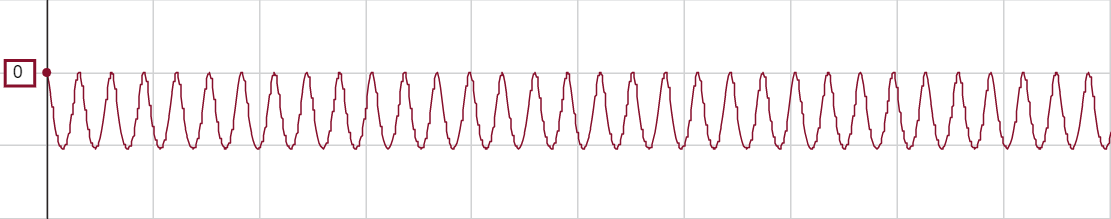
\includegraphics[scale=0.75]{pictures/control/posc}
    \end{center}
    \caption{An oscillating response with only gain in Simulink}
    \label{fig:posc}
\end{figure}

The measured $K_u$ and $T_u$, were plugged into the Ziegler-Nichols formula table (See table \ref{table.pidconstants}) and then fine-tuned to achieve less of an overshoot and faster response time.
The final values for an adjusted PID system where as follows, where red indicates the calculated values, and green - the fine-tuning. (See figure \ref{fig:simpidvalues})

\begin{figure}[H]
    \begin{center}
    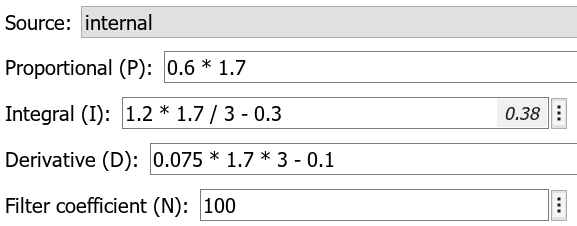
\includegraphics[scale=0.65]{pictures/control/simpidvalues}
    \end{center}
    \caption{Tuned PID controller block values}
    \label{fig:simpidvalues}
\end{figure}

After tuning the PID, the output response was
\begin{figure}[H]
    \begin{center}
    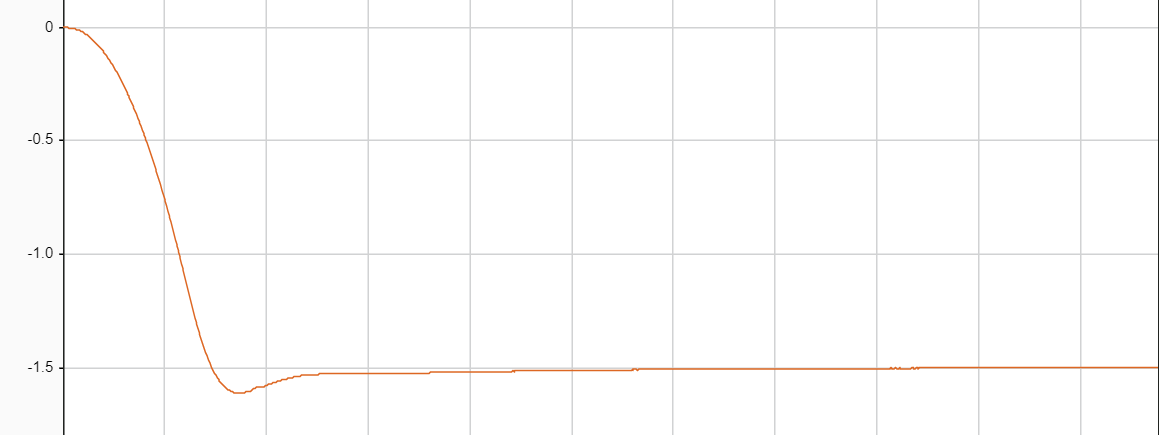
\includegraphics[scale=0.7]{pictures/control/zpidnonoise}
    \end{center}
    \caption{}
    \label{fig:zpidnonoise}
\end{figure}

\begin{figure}[H]
    \begin{center}
    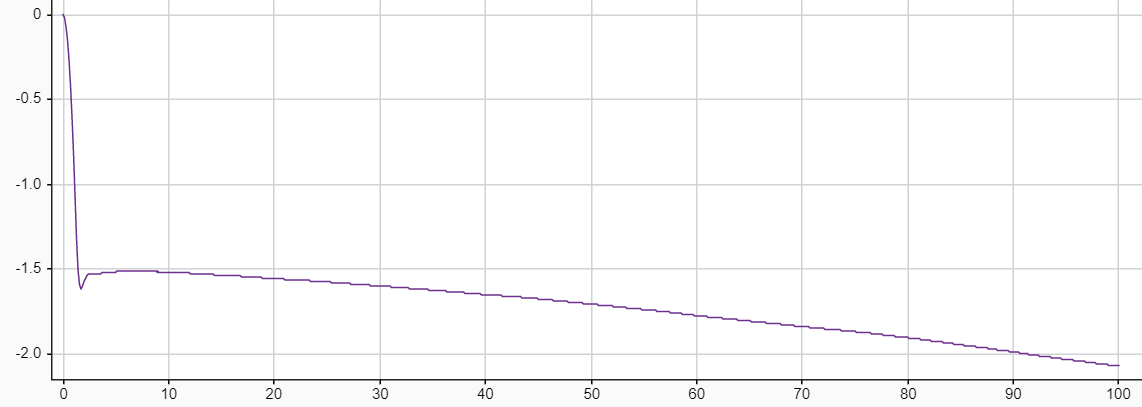
\includegraphics[scale=0.7]{pictures/control/zpidnoise}
    \end{center}
    \caption{Example of a system tuned using the Ziegler-Nichols method\cite{LibrePID}}
    \label{fig:zpidnoise}
\end{figure}

\begin{figure}[H]
    \begin{center}
    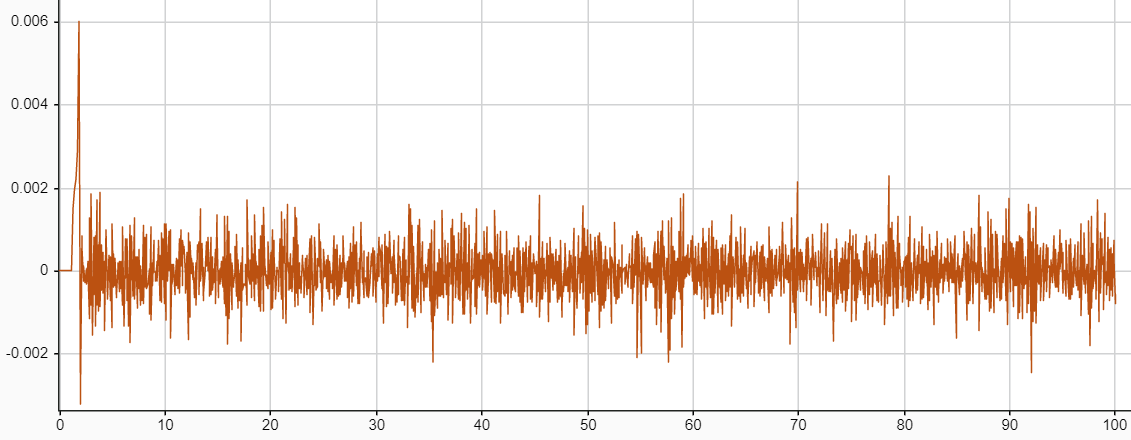
\includegraphics[scale=0.7]{pictures/control/phiPID.PNG}
    \end{center}
    \caption{Response of a tune phi/roll PID}
    \label{fig:phipid}
\end{figure}

\begin{figure}[H]
    \begin{center}
    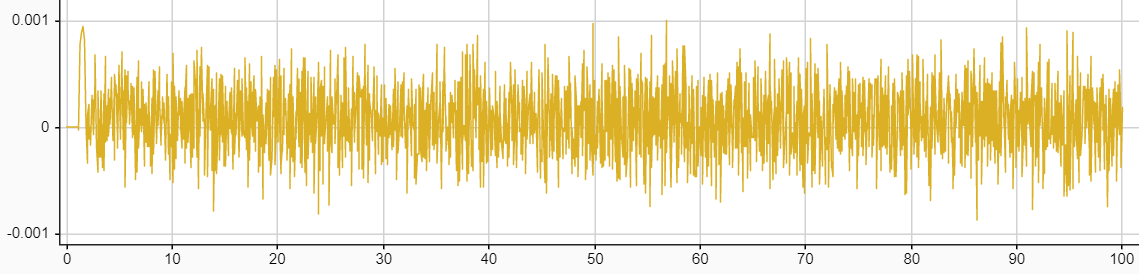
\includegraphics[scale=0.7]{pictures/control/thetaPID.PNG}
    \end{center}
    \caption{Response of a tune theta/pitch PID}
    \label{fig:thetapid}
\end{figure}